Librăria de șah are două elemente principale folosite în frontend:
structura \textit{Game} și funcția \textit{bot\_move}.

Structura \textit{Game} conține toate informațiile despre jocul curent și este definită astfel:
\begin{lstlisting}[language=RustHtml]
struct Game {
    board: Board,
    moves: Vec<Move>,
    fifty_move_rule: u8,
    game_state: GameState,
    board_history: Vec<Board>,
}
\end{lstlisting}

\begin{itemize}
	\item Câmpul \textit{board} conține configurația curentă de piese
	\item Câmpul \textit{moves} conține un vector cu mutările jucate până acum
	\item Câmpul \textit{fifty\_move\_rule} numără câte mutări au trecut de la ultima
	      mutare de pion sau captură (dacă ajunge la 50 jocul se declară remiză)
	\item Câmpul \textit{game\_state} memorează stadiul curent al jocului și poate lua
	      una dintre următoarele valori:
	      \begin{itemize}
		      \item InProgress
		      \item Checkmate
		      \item Stalemate (jucătorul curent nu poate face nicio mutare, dar nu este în șah.
		            Jocul se declară remiză)
		      \item DrawByRepetition (dacă se repetă aceeași poziție a pieselor de 3 ori jocul
		            se declară remiză)
		      \item DrawByFiftyMoveRule
		      \item DrawByInsufficientMaterial (dacă niciunul din jucători nu are destule piese
		            pentru a da mat jocul se declară remiză)
	      \end{itemize}
	\item Câmpul \textit{board\_history} conține configurațiile pentru fiecare mutare.
	      Este folosit pentru verificarea regulii de remiză prin repetiție și pentru
	      a afișa mai ușor istoricul jocului în frontend
\end{itemize}
\vspace{1cm}

Tabla de șah este alcătuită din 64 de pătrate, același număr ca numărul de biți pe care
îl folosesc procesoarele moderne. Astfel se poate asocia fiecărui pătrat un bit unic într-o
variabilă pe 64 de biți (de exemplu \textit{unsigned long long} in c++ sau \textit{u64} in Rust),
unde valoarea de 1 înseamnă că pătratul este ocupat de o piesă, iar 0 că este liber.

Nu este de ajuns, însă, să se memoreze toată tabla într-un singur număr, deoarece se pierde informația
despre tipul fiecărei piese, deci se țin minte 7 numere pentru fiecare culoare (pentru pioni, cai,
nebuni, ture, regine, rege și unul cu toate piesele combinate).

Această reprezentare se numește \textit{BitBoards} și este eficientă din punct de vedere al memoriei, dar, mai important, din punct
de vedere al timpului de executare, deoarece pentru generarea mutărilor sau obținerea informațiilor
despre tablă se folosesc operații pe biți.
\vspace{0.5cm}

Așadar structura \textit{Board} este definită astfel
(tipul \textit{BitBoard} este un număr pe 64 de biți):
\begin{lstlisting}[language=RustHtml]
struct Board {
    w_pawn: BitBoard,
    w_knight: BitBoard,
    w_bishop: BitBoard,
    w_rook: BitBoard,
    w_queen: BitBoard,
    w_king: BitBoard,
    b_pawn: BitBoard,
    b_knight: BitBoard,
    b_bishop: BitBoard,
    b_rook: BitBoard,
    b_queen: BitBoard,
    b_king: BitBoard,

    w_occ: BitBoard,
    b_occ: BitBoard,
    occ: BitBoard,

    side_to_move: Color,
    in_check: bool,

    en_passant: Option<Square>,
    can_castle: u8,
}
\end{lstlisting}
Pe lângă cele 14 numere precizate mai sus, structura mai are câteva câmpuri:
\begin{itemize}
	\item Câmpul \textit{occ} conține numărul care reprezintă toată tabla
	\item Câmpul \textit{side\_to\_move} conține jucătorul curent (\textit{White} sau \textit{Black})
	\item Câmpul \textit{in\_check} ține minte dacă jucătorul curent este în șah
	\item Câmpul \textit{en\_passant} ține minte dacă în ultima mutare un pion a avansat cu 2
	      pătrate și pătratul de pe care a plecat, pentru o regulă mai puțin cunoscută numita
	      en passant (dacă un pion s-a mutat 2 pătrate și ajunge în dreptul unui pion inamic
	      poate fi capturat de oponent \textbf{doar} pentru următoarea mutare)

	      \begin{center}
		      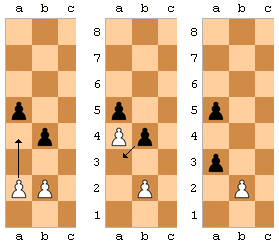
\includegraphics[width=5cm]{3/alg/en_passant.png}
	      \end{center}
	      \vspace{1cm}

	\item Câmpul \textit{can\_castle} ține minte folosind 2 biți pentru fiecare jucător dacă
	      poate face rocada, câte un bit pentru fiecare direcție.
\end{itemize}
\vspace{1cm}


Funcția \textit{bot\_move} calculează cea mai bună mutare pentru un \textit{Board} și o
dificultate anume pe care le primește ca parametrii.
Algoritmul de căutare a celei mai bune mutări este compus din 3 părți:
\begin{enumerate}
	\item Generarea mutărilor legale
	\item Evaluarea unei poziții
	\item Căutarea celei mai bune mutări
\end{enumerate}
